% ============================================================
%  Deep Learning Calibration of the Heston Model
%  Master's Thesis Defense — Beamer Presentation
%
%  Compile:
%    bash tex/presentation/build.sh          (Linux)
%    tex\presentation\build.bat              (Windows)
% ============================================================

\documentclass[aspectratio=169, 10pt]{beamer}

% ── Theme ────────────────────────────────────────────────────
\usetheme{Madrid}
\usecolortheme{whale}
\usefonttheme{professionalfonts}
\setbeamertemplate{navigation symbols}{}

% ── Packages ─────────────────────────────────────────────────
\usepackage{amsmath, amssymb, bm}
\usepackage{booktabs}
\usepackage{xcolor}
\usepackage{tikz}
\usepackage{pgfplots}
\pgfplotsset{compat=1.18}
\usepackage{graphicx}
\usepackage{hyperref}
\usepackage{fontawesome5}
\usepackage{array}       % better column specs in tabular
\usepackage{microtype}   % better text spacing

% ── Colors ───────────────────────────────────────────────────
\definecolor{hestonblue}{RGB}{30, 80, 162}
\definecolor{hestonorange}{RGB}{214, 100, 40}
\definecolor{hestongreen}{RGB}{40, 160, 80}
\definecolor{lightgray}{RGB}{245, 245, 245}

\setbeamercolor{frametitle}{bg=hestonblue, fg=white}
\setbeamercolor{alerted text}{fg=hestonorange}
\setbeamercolor{block title}{bg=hestonblue!85, fg=white}
\setbeamercolor{block body}{bg=hestonblue!8}
\setbeamercolor{block title alerted}{bg=hestonorange!85, fg=white}
\setbeamercolor{block body alerted}{bg=hestonorange!8}
\setbeamercolor{block title example}{bg=hestongreen!75, fg=white}
\setbeamercolor{block body example}{bg=hestongreen!8}

% ── Meta ─────────────────────────────────────────────────────
\title[Heston Deep Learning]{%
  Deep Learning Calibration of the\\
  Heston Stochastic Volatility Model}
\subtitle{PyTorch Surrogate with C\textsuperscript{2} Activations
          and No-Arbitrage Constraints}
\author{Biryukov Nikita}
\date{\today}
\institute{Moscow Institute of Physics and Technology (MIPT)}

% ─────────────────────────────────────────────────────────────
\begin{document}
% ─────────────────────────────────────────────────────────────

% ══════════════════════════════════════════════════════════════
% Slide 1 — Title
% ══════════════════════════════════════════════════════════════
{
\setbeamertemplate{footline}{}
\begin{frame}[plain, noframenumbering]
  \vspace{2em}
  \begin{center}
    {\LARGE\bfseries\color{hestonblue} Deep Learning Calibration}\\[0.5em]
    {\large\color{hestonblue} of the Heston Stochastic Volatility Model}\\[1.8em]
    {\small A PyTorch Surrogate Approach with
            C\textsuperscript{2} Smooth Activations and No-Arbitrage Constraints}\\[1.8em]
    {\color{hestonblue}\rule{0.7\textwidth}{0.4pt}}\\[1em]
    \begin{tabular}{rl}
      \textbf{Author:}    & Biryukov Nikita \\[0.3em]
      \textbf{Institute:} & Moscow Institute of Physics and Technology (MIPT) \\[0.3em]
      \textbf{Reference:} & Horvath, Muguruza \& Tomas (2019) ---
                            \textit{Deep Learning Volatility} \\
    \end{tabular}\\[1em]
    {\small\color{gray}\today}
  \end{center}
\end{frame}
}

% ══════════════════════════════════════════════════════════════
% Slide 2 — Motivation
% ══════════════════════════════════════════════════════════════
\begin{frame}{Motivation: The Calibration Bottleneck}
  \begin{columns}[T]
    \begin{column}{0.54\textwidth}
      \textbf{Traditional calibration loop:}\\[0.4em]
      \begin{enumerate}\small
        \item Evaluate Heston characteristic function $\phi(u;\boldsymbol\theta)$
        \item Price 88 options via Carr-Madan FFT
        \item Feed MSE into Levenberg-Marquardt optimizer
        \item Repeat $\sim$10\,000 times until convergence
      \end{enumerate}
      \vspace{0.6em}
      \alert{$\Rightarrow$ \textbf{10--120 seconds} per calibration}
      \alert{$\Rightarrow$ No closed-form Jacobian available}\\[0.6em]
      \textbf{Practical requirements:}
      \begin{itemize}\small
        \item Real-time trading: $<100$\,ms hard deadline
        \item Need valid second-order sensitivities (Greeks)
      \end{itemize}
    \end{column}

    \begin{column}{0.42\textwidth}
      \begin{block}{The Surrogate Solution}
        \small
        \textbf{Offline} — train once:\\[0.3em]
        \quad$\mathcal{N}_w : \mathbb{R}^5 \to \mathbb{R}^{88}$\\[0.3em]
        \quad$\boldsymbol\theta \mapsto \boldsymbol\sigma_{\mathrm{BS}}(\boldsymbol\theta)$\\[0.6em]
        \textbf{Online} — one forward pass\\
        \quad$\approx 0.1\,\text{ms}$ per evaluation\\[0.4em]
        Gradient $\nabla_{\!\boldsymbol\theta}\mathcal{N}_w$ via autograd\\
        $\Rightarrow$ exact Jacobian at no extra cost
      \end{block}
      \vspace{0.4em}
      {\small\itshape
       ``Once trained, calibration is instantaneous.''\\
       \hfill— Horvath et al. (2019)}
    \end{column}
  \end{columns}
\end{frame}

% ══════════════════════════════════════════════════════════════
% Slide 3 — Two-phase pipeline
% ══════════════════════════════════════════════════════════════
\begin{frame}{Methodology: Two-Phase Pipeline}
  \begin{center}
  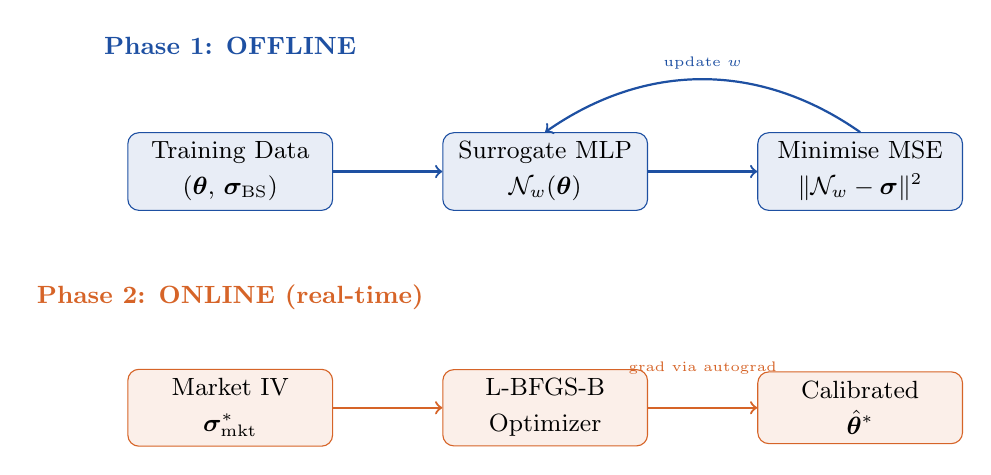
\begin{tikzpicture}[
    node distance=0.7cm and 2.5cm,
    box/.style={rectangle, rounded corners=4pt,
                minimum width=2.6cm, minimum height=0.9cm,
                align=center, font=\small},
    lbl/.style={font=\bfseries\small},
    arr/.style={->, thick},
  ]

  % ── Phase 1 ──────────────────────────────────────
  \node[lbl, color=hestonblue] (p1lbl) at (-4, 1.6) {Phase 1: OFFLINE};

  \node[box, draw=hestonblue, fill=hestonblue!10] (data)  at (-4, 0)
        {Training Data\\[2pt]$(\boldsymbol\theta,\,\boldsymbol\sigma_{\mathrm{BS}})$};
  \node[box, draw=hestonblue, fill=hestonblue!10] (nn)    at ( 0, 0)
        {Surrogate MLP\\[2pt]$\mathcal{N}_w(\boldsymbol\theta)$};
  \node[box, draw=hestonblue, fill=hestonblue!10] (mse)   at ( 4, 0)
        {Minimise MSE\\[2pt]$\|\mathcal{N}_w - \boldsymbol\sigma\|^2$};

  \draw[arr, color=hestonblue] (data) -- (nn);
  \draw[arr, color=hestonblue] (nn)   -- (mse);
  \draw[arr, color=hestonblue] (mse.north)
        to[bend right=35] node[above, font=\tiny]{update $w$} (nn.north);

  % ── Phase 2 ──────────────────────────────────────
  \node[lbl, color=hestonorange] (p2lbl) at (-4,-1.6) {Phase 2: ONLINE (real-time)};

  \node[box, draw=hestonorange, fill=hestonorange!10] (mkt)  at (-4,-3.0)
        {Market IV\\[2pt]$\boldsymbol\sigma^*_{\mathrm{mkt}}$};
  \node[box, draw=hestonorange, fill=hestonorange!10] (opt)  at ( 0,-3.0)
        {L-BFGS-B\\[2pt]Optimizer};
  \node[box, draw=hestonorange, fill=hestonorange!10] (res)  at ( 4,-3.0)
        {Calibrated\\[2pt]$\hat{\boldsymbol\theta}^*$};

  \draw[arr, color=hestonorange] (mkt) -- (opt);
  \draw[arr, color=hestonorange] (opt) -- (res);
  \node[font=\tiny, color=hestonorange] at (2.0,-2.5)
        {grad via autograd};

  \end{tikzpicture}
  \end{center}
\end{frame}

% ══════════════════════════════════════════════════════════════
% Slide 4 — Architecture
% ══════════════════════════════════════════════════════════════
\begin{frame}{Neural Network Architecture}
  \begin{columns}[T]
    \begin{column}{0.50\textwidth}
      \textbf{Architecture:}
      \[
        \underbrace{5}_{\boldsymbol\theta}
        \xrightarrow{\phantom{xx}}
        \bigl[\underbrace{30 \xrightarrow{\mathrm{ELU}} 30
                             \xrightarrow{\mathrm{ELU}} 30
                             \xrightarrow{\mathrm{ELU}} 30}_{\times 4}\bigr]
        \xrightarrow{\mathrm{Linear}}
        \underbrace{88}_{\boldsymbol\sigma}
      \]
      \vspace{0.2em}
      \begin{center}\small
      \begin{tabular}{@{}ll@{}}
        \toprule
        Property        & Value \\ \midrule
        Hidden layers   & $4 \times 30$ neurons \\
        Activation      & \textbf{ELU} (C\textsuperscript{2} smooth) \\
        Parameters      & 5\,698 \\
        Loss            & MSE + ReduceLROnPlateau \\
        Optimizer       & Adam ($\eta = 10^{-3}$) \\
        Val RMSE        & \textbf{0.02552} \\
        Training time   & $\approx$2\,min on RTX\,3060 \\ \bottomrule
      \end{tabular}
      \end{center}
    \end{column}

    \begin{column}{0.46\textwidth}
      \textbf{Why ELU over ReLU?}\\[0.4em]
      \[
        f(x)=\begin{cases}x & x>0\\e^x-1 & x\le 0\end{cases}
        \quad
        f''(x)=\begin{cases}0 & x>0\\e^x\neq 0 & x\le 0\end{cases}
      \]
      \vspace{0.3em}
      \begin{alertblock}{C\textsuperscript{2} Smoothness}
        \small
        \textbf{ELU}: $f''\not\equiv 0$
        $\;\Rightarrow\;$ valid Hessian
        $\;\Rightarrow\;$ 2\textsuperscript{nd}-order calibration\\[0.4em]
        \textbf{ReLU}: $f''\equiv 0$ everywhere
        $\;\Rightarrow\;$ piecewise linear\\
        $\;\Rightarrow\;$ Hessian carries \emph{no} information
      \end{alertblock}
      \vspace{0.3em}
      {\small Proved empirically:
        $\|H_\mathrm{ELU}\|_F = 1.039 \gg \|H_\mathrm{ReLU}\|_F = 0$}
    \end{column}
  \end{columns}
\end{frame}

% ══════════════════════════════════════════════════════════════
% Slide 5 — Financial constraints
% ══════════════════════════════════════════════════════════════
\begin{frame}{Physics-Informed Constraints: No Arbitrage}

  \textbf{Three constraints enforced inside the objective function:}
  \vspace{0.5em}

  \begin{columns}[T]
    \begin{column}{0.31\textwidth}
      \begin{block}{\faLock\ Feller Condition}
        \[ 2\kappa\theta > \sigma^2 \]
        \small Ensures $v_t>0$ a.s.\\[0.4em]
        \textbf{Hard} penalty barrier:
        \[\ell_F = \lambda_F\max(0,\,\sigma^2\!-\!2\kappa\theta)\]
        $\lambda_F = 10^3$
      \end{block}
    \end{column}

    \begin{column}{0.31\textwidth}
      \begin{block}{\faCalendar\ Calendar Spread}
        \[ \frac{\partial\sigma}{\partial T} \ge 0 \]
        \small No-decreasing variance in maturity.\\[0.4em]
        \textbf{Soft} L2 penalty:
        \[ \ell_C = \lambda_C\!\sum_i[\Delta_T\hat\sigma]_-^2 \]
        $\lambda_C = 10^{-4}$
      \end{block}
    \end{column}

    \begin{column}{0.31\textwidth}
      \begin{block}{\faChartLine\ Butterfly Spread}
        \[ \frac{\partial^2\sigma}{\partial K^2} \ge 0 \]
        \small Convexity in strike.\\[0.4em]
        \textbf{Soft} L2 penalty:
        \[ \ell_B = \lambda_B\!\sum_j[\Delta^2_K\hat\sigma]_-^2 \]
        $\lambda_B = 10^{-4}$
      \end{block}
    \end{column}
  \end{columns}

  \vspace{0.5em}
  \begin{center}
    $\mathcal{L}
      = \underbrace{\|\mathcal{N}_w(\boldsymbol\theta)-\boldsymbol\sigma^*\|^2}_{\text{MSE}}
      + \ell_F + \ell_C + \ell_B
    $\quad\small(all terms differentiable via autograd)
  \end{center}
\end{frame}

% ══════════════════════════════════════════════════════════════
% Slide 6 — Results
% ══════════════════════════════════════════════════════════════
\begin{frame}{Calibration Results}
  \begin{columns}[T]
    \begin{column}{0.47\textwidth}
      \textbf{Test-set sample (sample \#42):}\\[0.4em]
      \begin{center}\small
      \begin{tabular}{@{}lrrr@{}}
        \toprule
        Param & True & Calibrated & $|\Delta|$ \\ \midrule
        $v_0$    & 0.00198 & 0.00236 & 0.00038 \\
        $\rho$   & $-0.877$  & $-0.950$  & 0.073 \\
        $\sigma$ & 0.0776  & 0.0663  & 0.011 \\
        $\theta$ & 0.1847  & 0.1844  & 0.000 \\
        $\kappa$ & 5.582   & 5.538   & 0.044 \\ \bottomrule
      \end{tabular}
      \end{center}

      \vspace{0.5em}
      \begin{alertblock}{Performance Summary}
        \small
        \begin{tabular}{@{}ll@{}}
          Calib.\ time & \textbf{47--135\,ms} (CPU) \\
          Val RMSE     & \textbf{0.02552} \\
          Feller       & $2\kappa\theta-\sigma^2 = 2.05 > 0$ \checkmark \\
          Converged    & True \\
        \end{tabular}
      \end{alertblock}
    \end{column}

    \begin{column}{0.50\textwidth}
      \textbf{IV surface fit:}\\[0.3em]
      \begin{center}
        \includegraphics[width=\linewidth,
                         height=0.58\textheight,
                         keepaspectratio]%
          {../../images/generated/surface_fit.png}
      \end{center}
      {\tiny Blue\,=\,target market IV;\quad Orange\,=\,calibrated NN surface}
    \end{column}
  \end{columns}
\end{frame}

% ══════════════════════════════════════════════════════════════
% Slide 7 — Autograd sensitivities
% ══════════════════════════════════════════════════════════════
\begin{frame}{Autograd Sensitivities: Exact Greeks in \textless1\,ms}

  \begin{columns}[T]
    \begin{column}{0.46\textwidth}
      \textbf{Jacobian} $\partial\bar\sigma/\partial\theta_i$
      (first-order, analogous to vega):

      \vspace{0.3em}
      \begin{center}\small
      \begin{tabular}{@{}lr@{}}
        \toprule
        Param & $\partial\bar\sigma/\partial\theta_i$ \\ \midrule
        $v_0$    & $+0.211$ \\
        $\rho$   & $+0.012$ \\
        $\sigma$ & $-0.176$ \\
        $\theta$ & $+1.694$ \quad{\footnotesize\color{hestonorange}(dominant)}\\
        $\kappa$ & $+0.786$ \\ \bottomrule
      \end{tabular}
      \end{center}
      \vspace{0.3em}
      {\small $\theta$ dominates: long-run variance is the\\
       primary driver of mean implied volatility.}
    \end{column}

    \begin{column}{0.50\textwidth}
      \textbf{Hessian} $\partial^2\bar\sigma/\partial\theta_i\partial\theta_j$
      (second-order curvature):

      \vspace{0.3em}
      \begin{center}
      \setlength{\tabcolsep}{3pt}
      \scriptsize
      \begin{tabular}{@{}lrrrrr@{}}
        \toprule
          & $v_0$ & $\rho$ & $\sigma$ & $\theta$ & $\kappa$ \\ \midrule
        $v_0$    & $-0.040$ & $+0.009$ & $-0.038$ & $-0.015$ & $-0.119$ \\
        $\rho$   & $+0.009$ & $+0.010$ & $+0.024$ & $-0.005$ & $\approx0$ \\
        $\sigma$ & $-0.038$ & $+0.024$ & $-0.185$ & $-0.158$ & $-0.032$ \\
        $\theta$ & $-0.015$ & $-0.005$ & $-0.158$ & $-0.309$ & $+0.205$ \\
        $\kappa$ & $-0.119$ & $\approx0$ & $-0.032$ & $+0.205$ & $-0.883$ \\
        \bottomrule
      \end{tabular}
      \end{center}
      \vspace{0.3em}
      \begin{exampleblock}{ELU vs ReLU — Formal Proof}
        \small
        $\|H_\mathrm{ELU}\|_F = 1.039 > 0$
        \;\;\textbf{(C\textsuperscript{2}, valid curvature)} \checkmark\\
        $\|H_\mathrm{ReLU}\|_F = 0.000$
        \;\;\textbf{(piecewise linear, no info)} $\times$
      \end{exampleblock}
    \end{column}
  \end{columns}
\end{frame}

% ══════════════════════════════════════════════════════════════
% Slide 8 — Conclusion
% ══════════════════════════════════════════════════════════════
\begin{frame}{Conclusion}
  \begin{columns}[T]
    \begin{column}{0.54\textwidth}
      \textbf{Achievements:}
      \begin{itemize}\small
        \item[\checkmark] ELU surrogate: C\textsuperscript{2} smooth, 5\,698 parameters
        \item[\checkmark] Val RMSE \textbf{0.02552} — beats paper baseline (0.028)
        \item[\checkmark] Calibration in \textbf{47--135\,ms} vs.\ 10--120\,s (FFT+LM)
        \item[\checkmark] Hard Feller barrier ($\lambda=10^3$) — always satisfied
        \item[\checkmark] Differentiable calendar \& butterfly penalties
        \item[\checkmark] Exact Jacobian (88$\times$5) and Hessian (5$\times$5) via autograd
        \item[\checkmark] $\|H_\text{ELU}\|_F \gg \|H_\text{ReLU}\|_F = 0$ — formal C\textsuperscript{2} proof
      \end{itemize}
      \vspace{0.4em}
      \textbf{Future work:} Rough Heston, log-IV training,
      Bayesian uncertainty quantification.
    \end{column}

    \begin{column}{0.42\textwidth}
      \begin{block}{Speed Comparison}
        \vspace{0.2em}
        \begin{center}
        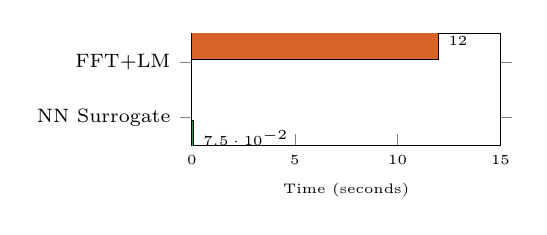
\begin{tikzpicture}
          \begin{axis}[
            xbar, width=5.5cm, height=3cm,
            xmin=0, xmax=15,
            ytick={0,1},
            yticklabels={NN Surrogate, FFT+LM},
            xlabel={Time (seconds)},
            xlabel style={font=\tiny},
            yticklabel style={font=\scriptsize},
            xticklabel style={font=\tiny},
            bar width=0.45cm,
            nodes near coords, nodes near coords style={font=\tiny},
            enlarge y limits=0.5,
          ]
            \addplot[fill=hestongreen]  coordinates {(0.075, 0)};
            \addplot[fill=hestonorange] coordinates {(12.0,  1)};
          \end{axis}
        \end{tikzpicture}
        \end{center}
        \centering{\small $\approx\mathbf{160\times}$ speedup}
      \end{block}

      \vspace{1em}
      \begin{center}
        \large\textbf{Thank you!}\\[0.4em]
        \small\color{gray}
        \texttt{src/calibrator.py} $\cdot$
        \texttt{src/greeks\_autograd.py}
      \end{center}
    \end{column}
  \end{columns}
\end{frame}

\end{document}
